\documentclass[12pt,letterpaper]{hmcpset}
\usepackage[margin=1in]{geometry}
\usepackage{graphicx}
\usepackage{zach}
\usepackage{drawstack}
\usepackage{tabu}

% info for header block in upper right hand corner
\name{Zachary Seymour}
\class{CS 571}
\assignment{Assignment 2}
\duedate{October 14, 2013}

\begin{document}



\begin{problem}[1]
Given the C program....
\end{problem}

\begin{problem}[1a]
Does the program produce dangling references? Why?
\end{problem}
\begin{solution}
There is no call to \texttt{free} and all the code is running in the same scope, so no dangling references are produced.
\end{solution}

\begin{problem}[1b]
Does the program produce garbage? Why?
\end{problem}
\begin{solution}
The program does not produce garbage.
\end{solution}

\begin{problem}[2]
Give the output of the following program (in pseudo-code) using the two parameter passing methods (call by value/reference).
\end{problem}
\begin{solution}
\begin{itemize}
\item Call-by-value:

\verb|2 1 0|

\verb|2 1 0|

\item Call-by-reference:

\verb|2 1 0|

\verb|2 1 0|
\end{itemize}
\end{solution}


\begin{problem}[3]
For the following C program....
\end{problem}

\begin{problem}[3a]
Draw the stack activation records after the call to \texttt{r} on line 13.
\end{problem}

\begin{solution}
\begin{drawstack}
\startframe
\cell{global var \code{int x}}
\finishframe{COMMON area}
\startframe
\cell{\code{main}}
\finishframe{activation record of \code{main}}
\startframe
\cell{control link} \link{1}
\cell{return address}
\cell{var \code{double x}}
\finishframe{activation record of \code{q}}
\startframe
\cell{control link} \link{3}
\cell{return address}
\finishframe{activation record of \code{r}}
\end{drawstack}
\end{solution}

\begin{problem}[3b]
Draw the stack activation records after the call to \texttt{p} on line 14.
\end{problem}

\begin{solution}
\begin{drawstack}
\startframe
\cell{global var \code{int x}}
\finishframe{COMMON area}
\startframe
\cell{\code{main}}
\finishframe{activation record of \code{main}}
\startframe
\cell{control link} \link{1}
\cell{return address}
\cell{var \code{double x}}
\finishframe{activation record of \code{q}}
\startframe
\cell{control link} \link{3}
\cell{return address}
\cell{var \code{double r}}
\finishframe{activation record of \code{p}}
\end{drawstack}
\end{solution}

\begin{problem}[3c]
Describe where variables \texttt{r} and \texttt{x} are located on lines 4 and 5 and how they are accessed during the execution of p.
\end{problem}

\begin{solution}
The variable \code{r} is found with in the activation record from of \code{p}, so it is accessed by its offset within the frame.  The variable \code{x} is global, so it is found and accessed in the COMMON area before the activation frame of \code{main}.
\end{solution}

\begin{problem}[4]
To model the run-time semantics of procedures, it is known that a stack is generally needed. 
\end{problem}

\begin{problem}[4a]
If the language does not allow procedure recursion, do we have to have stacks? Why?
\end{problem}

\begin{solution}
If no function can be called inside another, there would not be a need for a stack.  We would either have one big activation record, containing the whole program or, perhaps, a linked-list of records, functions called one after the other, sharing and mutating common data.
\end{solution}

\begin{problem}[4b]
If the language does allow procedure recursion, but a recursive call can only happen at the end of a procedure, do we have to have stacks? Why?
\end{problem}

\begin{solution}
This is in fact the benefit of tail-call recursion so common in functional languages.  Since the recursive call is the last step in the function, nothing reaming in the activation frame is really needed.  We can just replace the old activation record with the new one.
\end{solution}

\begin{problem}[5]
Read the following Java code:
\end{problem}

\begin{problem}[5a]
After Line 0 is executed, does the heap create one continuous area with x, y, and color fields inside, or does the heap create two distinct areas, one with x, y and the other with color?
\end{problem}

\begin{solution}
One continuous area is created with the entry for color immediately following x and y.
\end{solution}

\begin{problem}[5b]
Suppose Line 1 is included in the program but Lines 2, 3, 4 are commented out, should the program compile? If not, why? If yes, what is the value of field x of pa? 
\end{problem}

\begin{solution}
The program will not compile as a Point cannot assigned to a ColorPoint without a cast declaration.
\end{solution}

\begin{problem}[5c]
Suppose Line 2 is included in the program but Lines 1, 3, 4 are commented out, should the program compile? If not, why? If yes, what is the value of field x of pb?
\end{problem}

\begin{solution}
Now, the program will compile, and we have \code{pb.x} equal to 1.
\end{solution}

\begin{problem}[5d]
Suppose Line 3 is included in the program but Lines 1, 2, 4 are commented out, should the program compile? If not, why? If yes, what would be run-time behavior of the program?
\end{problem}

\begin{solution}
The program does now compile, since the cast is made explicit; however, a \code{ClassCastException} is thrown at runtime.
\end{solution}

\begin{problem}[5e]
Suppose Line 4 is included in the program but Lines 1, 2, 3 are commented out, should the program compile? If not, why? If yes, what would be run-time behavior of the program?
\end{problem}

\begin{solution}
This compiles and behaves in the same way as part (c) because the cast is redundant.
\end{solution}

\begin{problem}[6]
Given the following C++ declarations, draw the VMT of each class and the layout of memory for a dynamically allocated object of \emph{each class}. 
\end{problem}

\begin{solution}
\begin{itemize}
\item VMT for class \code{A}

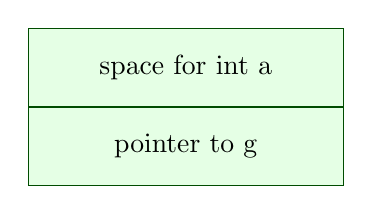
\begin{tikzpicture}
\cell{space for \code{int a}}
\cell{pointer to \code{g}}
\end{tikzpicture}
\item VMT for class \code{B}

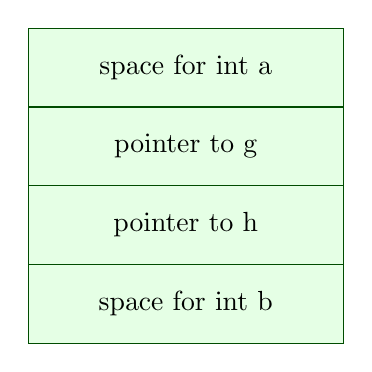
\begin{tikzpicture}
\cell{space for \code{int a}}
\cell{pointer to \code{g}}
\cell{pointer to \code{h}}
\cell{space for \code{int b}}
\end{tikzpicture}
\item VMT for class \code{C}

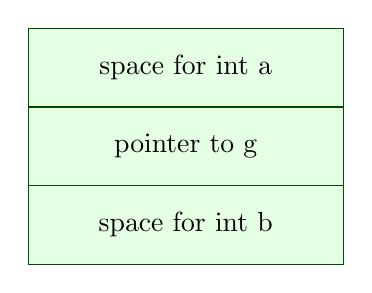
\begin{tikzpicture}
\cell{space for \code{int a}}
\cell{pointer to \code{g}}
\cell{space for \code{int b}}
\end{tikzpicture}

\item Memory layout for object of type \code{A}

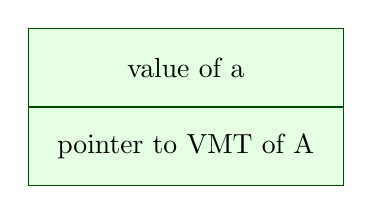
\begin{tikzpicture}
\cell{value of \code{a}}
\cell{pointer to VMT of \code{A}}
\end{tikzpicture}
\item Memory layout for object of type \code{B}

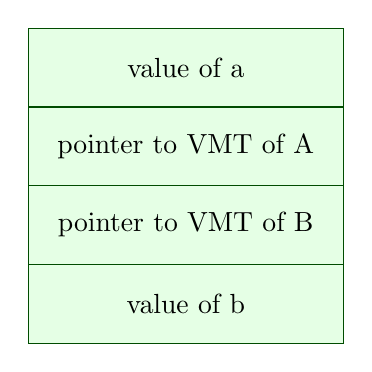
\begin{tikzpicture}
\cell{value of \code{a}}
\cell{pointer to VMT of \code{A}}
\cell{pointer to VMT of \code{B}}
\cell{value of \code{b}}
\end{tikzpicture}
\item Memory layout for object of type \code{C}

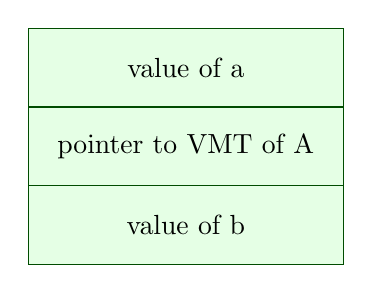
\begin{tikzpicture}
\cell{value of \code{a}}
\cell{pointer to VMT of \code{A}}
\cell{value of \code{b}}
\end{tikzpicture}
\end{itemize}
\end{solution}

\begin{problem}[7]
Many people think the Java ``interface'' mechanism is an encapsulation mechanism.  Their arguments are as follows. Suppose we have an interface A, being implemented by class B. If programmers consistently use type A every time an instance of B is referred to, then any method, say m, defined in B but not specified in A is hidden and cannot be accessed by any code holding a reference of type A. There however is a fatal flaw in this argument. Explain how a piece of code referring to an instance of B (with type A) can in fact access m.
\end{problem}

\begin{solution}
Provided the object is a true instance of B just having type A, the A object can be cast at runtime to a B object, and the method can validly be called.
\end{solution}

\begin{problem}[8]
Given the following Featherweight Java class definition:
\begin{verbatim}
class A extends Object 
{ 
    A() { super(); } 
} 

class B extends Object 
{ 
    B() { super(); } 
} 

class Pair extends Object 
{ 
    Object fst; 
    Object snd; 
    Pair(Object fst, Object snd) { super(); this.fst=fst; this.snd=snd; } 
    Pair setfst(Object newfst) { return new Pair(newfst, this.snd);} 
} 
\end{verbatim}
\end{problem}

\begin{problem}[8a]
Is it valid to write the following class:
\begin{verbatim}
class MyPair extends Pair
{
     MyPair(Object fst, Object snd) { super(fst, snd); } 
     Pair setfst(Object newfst) { return new MyPair(newfst, this.snd); } 
}
\end{verbatim}
If so, write a type derivation for method declaration \verb|Pair setfst(Object newfst) { return new MyPair(newfst, this.snd); }| If not, explain why.
\end{problem}

\begin{solution}
We must make all of the checks for method typing to insure this method is OK in class C.  First check is $\bar{\mathtt{x}}:\bar{\mathtt{C}}, \mathtt{this}:\mathtt{C}\vdash \mathtt{e_0}:\mathtt{E_0}$. So, given that all of the arguments are of the correct type and \code{this} is of type \code{MyPair}, then the return value has type $\mathtt{E_0}$, which should be a subtype of the return type, \code{Pair}.  Since \code{MyPair} is a subtype of \code{Pair} and \code{newfst} is of type \code{Object}, this condition checks out.  Since the \code{setfst} of \code{Pair} and \code{MyPair} take the same type of parameters and return the same type, the last criterion is met as well, so this method is valid and of type \code{Pair}.
\end{solution}

\begin{problem}[8b]
How does the following expression reduce? Please write it down step by step until no more reduction is possible:
\begin{verbatim}
new Pair(
         (new Pair(new A(), new B()).setfst(new B())).snd,
         (new Pair(new A(), new B()).setfst(new B())).fst
        )
\end{verbatim}
\end{problem}

\begin{solution}
\code{new Pair(\underline{(new Pair(new A(), new B()).setfst(new B())}).snd, (new Pair(new A(), new B()).setfst(new B())).fst)} \\
$\rightarrow$ \code{new Pair(new Pair(new A(), new B()).snd, \underline{(new Pair(new A(), new B()).setfst(new B())}).fst)} \\
$\rightarrow$ \code{new Pair(\underline{new Pair(new A(), new B()).snd}, new Pair(new A(), new B()).fst)} \\
$\rightarrow$ \code{new Pair(new B(), \underline{ new Pair(new A(), new B()).fst)}} \\
$\rightarrow$ \code{new Pair(new B(), new A())} \
\end{solution}


\end{document}
